\section{Economic Design of the NAX Token}
\subsection{Design Goal}
In addition to forming a positive economic game and increasing ecosystem activity, the goals of the public chain token economics should also conform to certain principles such as fair benefits, positive incentives, logical simplicity while being capalbe of utilization in diverse scenarios. The public token economy requires fair access to scenarios and diverse consumption scenarios while retaining a high holding value thereby promoting the development and growth of the public chain making the entire ecosystem more dynamic. To sum up, the design goals of NAX include:

\begin{enumerate}[\hspace{2cm}(a)]
    \item fair benefits
    \item positive incentives
    \item simple and effective
    \item retains high utility
\end{enumerate}

\subsection{Core Mechanism}

\subsubsection{Asset Fairness}
The effectiveness of a public chain's token economy comes from the fairness and legitimacy of asset acquisition. The requirements for acquiring assets should be simple, transparent and an identical process for the vast majority of people. In the Nebulas economy, NAS assets owned by users are relatively fair and legitimate and due to this, the primary way to obtain equity of a token is via Pledging (staking) NAS. Equity obtainment must not be due to unclear requirements or loopholes existing which lead to the phenomenon of poor asset allocation. The overall result of obtainment must be conducive to improved ecosystem development on the public chain.

\subsubsection{Decentralized pledge - dStaking}
The traditional centralized pledge method requires users to transfer assets into smart contracts for temporary custody. Asset security issues are maintained in a smart contract and unfortunately, smart contract asset security issues are common in the history of blockchain where hackers exploit contract loopholes and as a result the investors suffer large economic loss. 

Due to this, pledging also puts great pressure on public chain project parties since a large number of assets are kept in a smart contract which makes them targets. Due to this, the management and security of smart contracts is a large development bottleneck. All assets on the blockchain are genuine and pledging simply locks in the liquidity of that asset - it does not validate the ownership of the asset (although it can be retrieved by calling the contract method) once transferred to the contract.

We propose a new mechanism of pledging: dStaking (decentralized Staking) as shown in the figure \ref{fig:dStaking}. This new method ensures the assets are still owned by the user; the user enters into a pledge "contract" where the smart contract records the value of the pledge. The purpose of a pledge contract is simply to randomly verify whether the user is still fulfilling their contractual duties (e.g. pledging a minimum amount of NAS). When the balance of the pledging address is greater than or equal to the amount specified within the contract, it is considered a valid pledge, otherwise it will be considered a canceled pledge. The user is also able to add assets to their pledge and the system recalculates an average age based on the new pledge value which is discussed in the appendix.

The advantages of dStaking include:
\begin{enumerate}[\hspace{2cm}(a)]
    \item Protects user identification of assets
    \item Improve pledge paritipation due to eliminated security risk
    \item Improve overall asset security
\end{enumerate}

\begin{figure}[htbp]
  \centering
  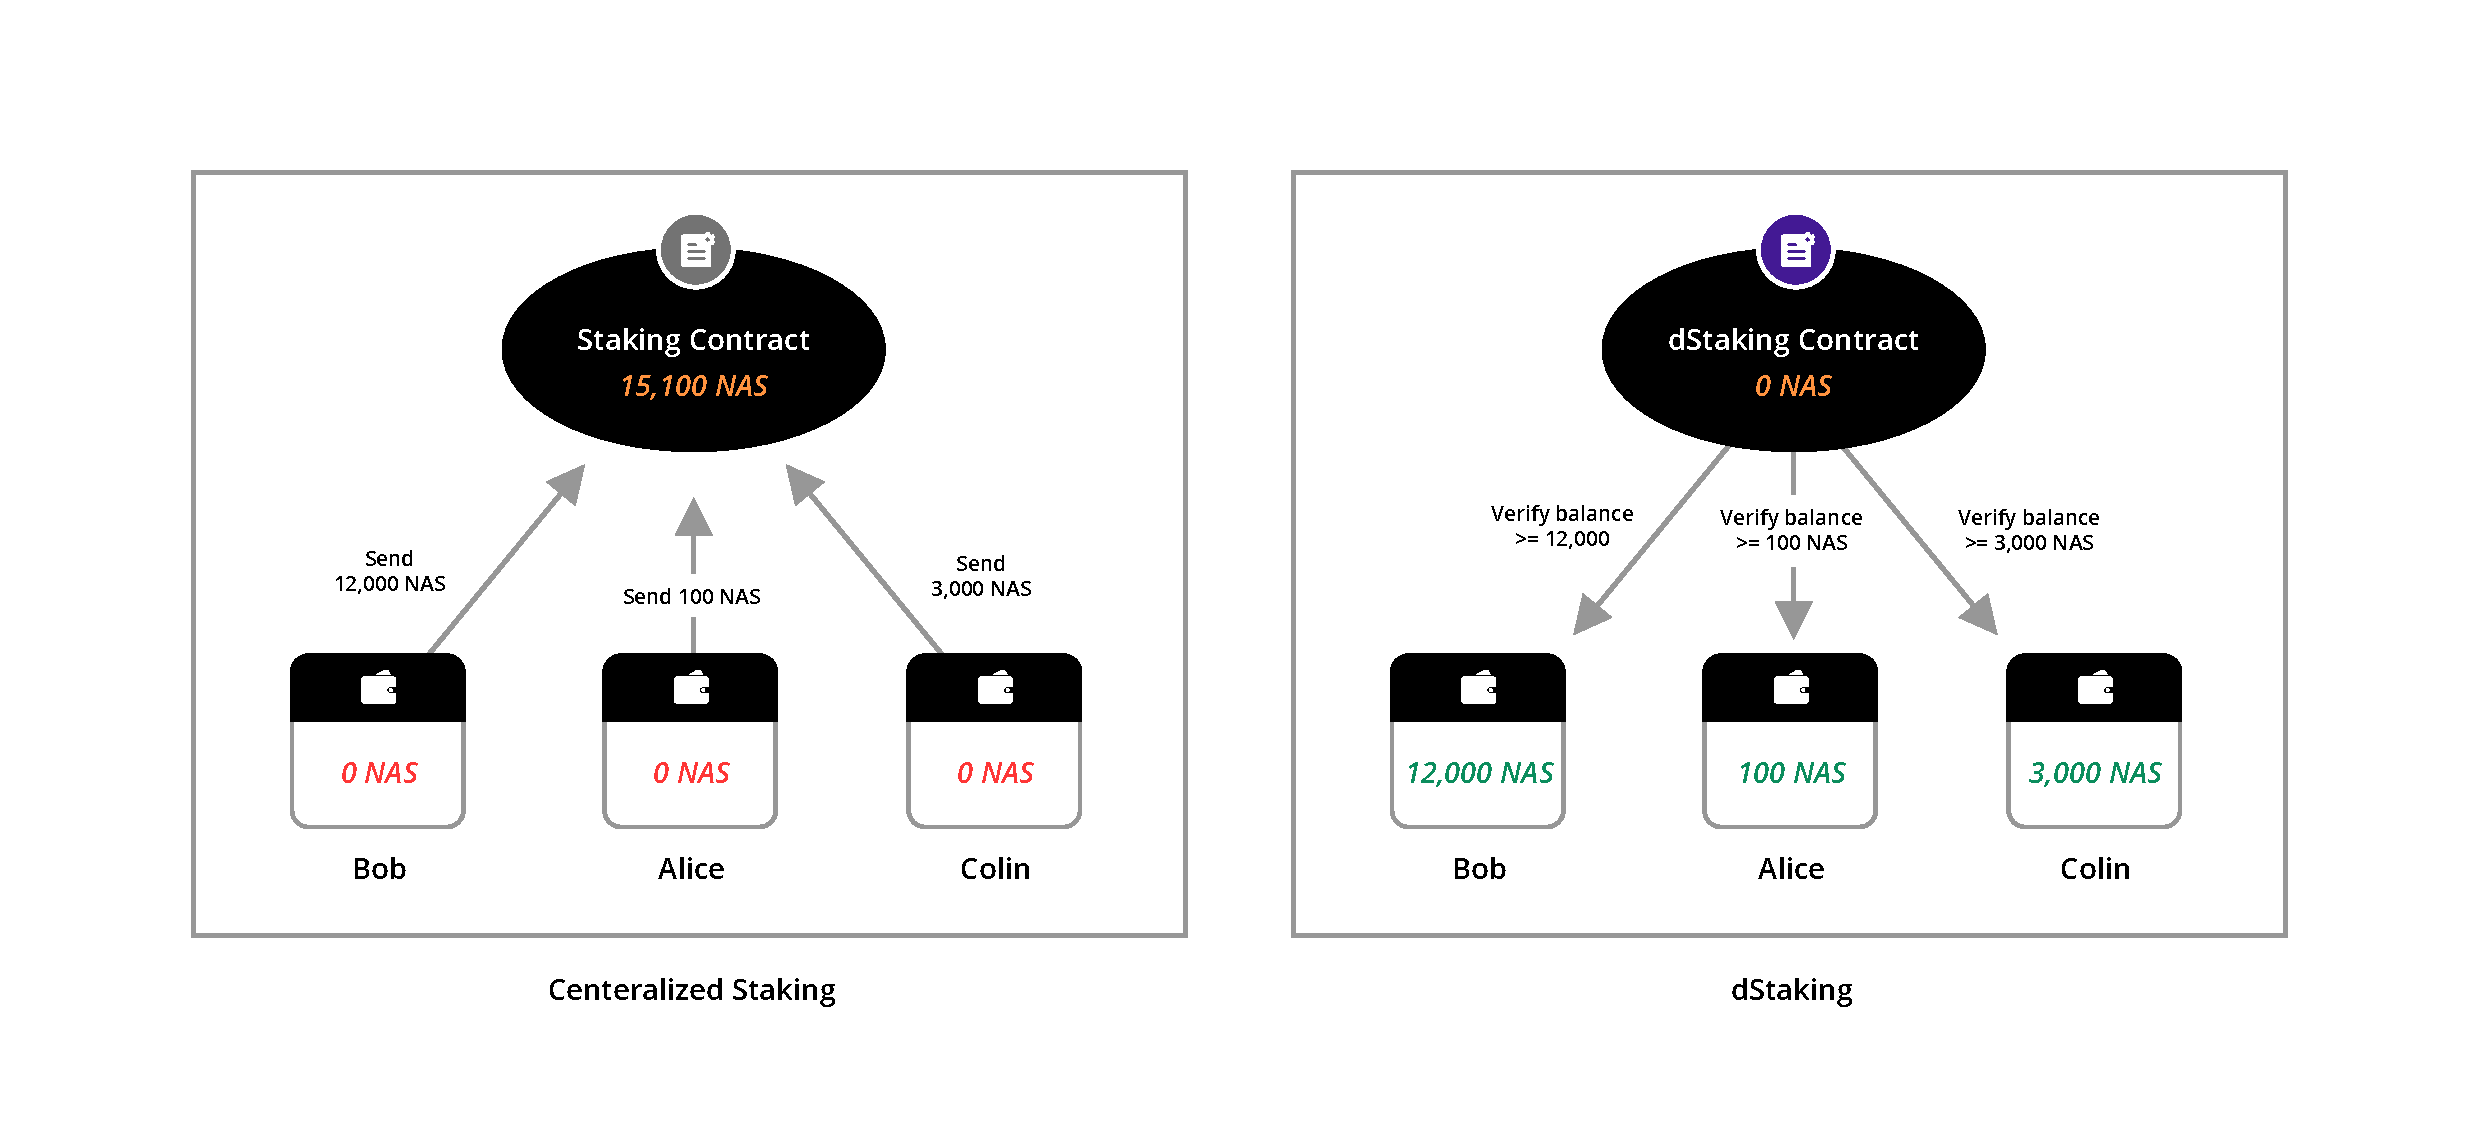
\includegraphics[width=1\textwidth]{../common/dStaking.pdf}
  \caption{Centralized pledge vs decentralized pledge\label{fig:dStaking}}
\end{figure}

\subsubsection{NAX Distribution Model - NDM}
As mentioned above, on the basis of safeguarding the equity and legitimacy of assets, and ensuring the inviolable ownership of pledged assets, the user contributes the liquidity of their assets and in return, they obtain corresponding ecological rights and interests. We call this new mode of token issuance "NDM" (Nebulas Devotional Mining). 

The maximum amount of NAX tokens that will be released is 10 billion(\(10^{10}\)) with an issuance cycle of every 6,000 blocks (approximately once per day tokens will be distributed). The number of tokens issued per cycle decreases with an attenuation coefficient of $\mu=0.999$ (reduction of 0.001\% every cycle) which leads to distribution completion in about 12 years. The number of pre-release NAX increases with the number of cycles, as shown in \ref{dist} and the cumulative number of pre-release NAXs is shown in \ref{acc}.

\begin{figure}[h]
\centering
\begin{minipage}[5cm]{.45\textwidth}
\centering
    \begin{tikzpicture}[scale=0.8]
    \begin{axis}[
        Axis lines = left,
        Xlabel = {number of cycles},
        Ylabel = {pre-release number of NAX},
    ]
    \addplot [
        Domain=-0:4000, 
        Samples=1000,
        Color=red,
    ]
    {1.0*10^7*0.999^x};

    \end{axis}
    \end{tikzpicture}
\caption{Pre-release number and period relationship}\label{dist}

\vspace{\baselineskip}
\end{minipage}\qquad
\begin{minipage}[5cm]{.45\textwidth}
\centering
    \begin{tikzpicture}[scale=0.72]
    \begin{axis}[
        Axis lines = left,
        Xlabel = {number of cycles},
        Ylabel = {accumulate pre-release NAX quantity},
    ]
    \addplot [
        Domain=-0:4000,
        Samples=1000, 
        Color=red,
    ]
    {10^10*(1 - 0.999^(x+1))};

    \addplot [
        Domain=-0:4000, 
        Samples=1000,
        Color=blue,
    ]
    {10^10};
    \end{axis}
    \end{tikzpicture}
\caption{cumulative pre-release quantity and period relationship}\label{acc}
\end{minipage}
\end{figure}

\subsubsection{Dynamic Distribution Model}
The dynamic distribution model refers to fact that the system will determine the actual number of NAX to be distributed according to specific variables with the intention to promote a positive economic game. At the beginning of NAX, we will introduce the pledge rate impact factor and dynamically adjusted the actual distribution ratio based on the increase or decrease of the pledge rate. In the future, we will introduce more  factors as needed. As shown in the figure \ref{fig:dynamic_dist}, the system pre-distributes $C_i$ NAX to the users pledging in the current period within the period $i$. In the actual distribution process, according to the current pledge rate level $\lambda$ (total amount of pledge NAS/total NAS circulation, 0<$\lambda$<1), the actual distribution of NAX is: $C_0 \mu ^i\lambda$.

\begin{figure}[h]
  \centering
  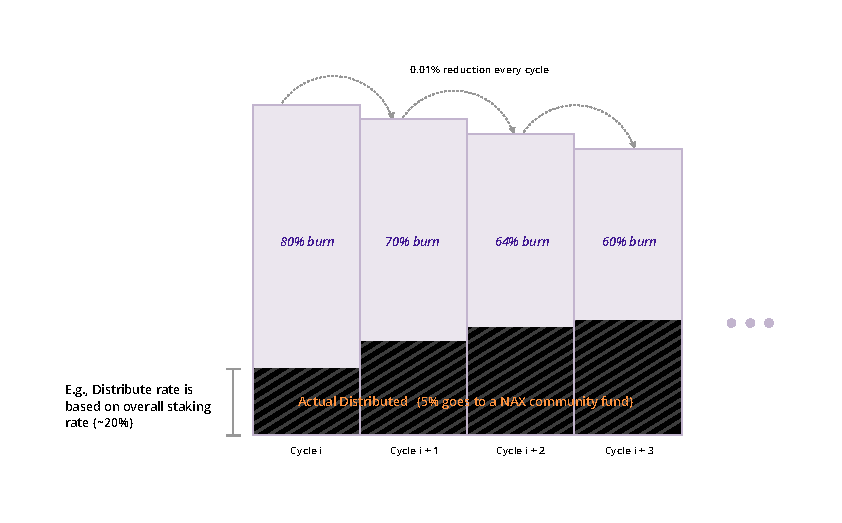
\includegraphics[width=0.8\textwidth]{../common/dynamic_dist.pdf}
  \caption{Dynamic distribution strategy diagram\label{fig:dynamic_dist}}
\end{figure}

\subsubsection{Distribution cycle}
During a distribution cycle, different number of pledge cycles will result in different distribution weights. The system determines the final NAX distribution amount based on the pledge quantity of each pledged user $V_{i, j}$ and the pledge weight \(f(T_{i, j})\). If the $N$ address is being validly pledged during the $i$ period, the $j$ address pledge is $V_{i,j}$, and the effective pledge period is $T_{i,j}$. Therefore, the number of NAXs that the address can be distributed to is $K_{i,j}$ as shown in the following formula.

\begin{equation}
  K_{i,j} = \frac{V_{i,j} f(T_{i,j})}{\sum_j V_{i,j} f(T_{i,j})} \lambda_i C_i
\end{equation}

Where \(f(T_{i,j})\) is the effective weight function for the pledge of the \(i\) user\(j\). The relationship between the pledge weight and the number of pledge cycles is as follows (the function relationship is shown in \ref{weight}).
\begin{equation}
  f(T) = 1 - \frac{\sqrt{(aT+b)^2+c^2}-(aT+b)}{2}
\end{equation}

\begin{figure}[h]
\centering
    \begin{tikzpicture}[scale=0.75]
    \begin{axis}[
        Axis lines = left,
        Xlabel = {number of pledge cycles},
        Ylabel = {effective weight},
    ]
    \addplot [
        Domain=0:365,
        Samples=200,
        Color=blue,
    ]
    {1-(sqrt((0.005*x-0.3)^2+0.2^2)-(0.005*x-0.3))/2};

    \addplot [
        Domain=-0:365, 
        Samples=200, 
        Color=red,
    ]
    {1};
    \end{axis}
    \end{tikzpicture}
\caption{Relationship between the effective weight of the pledge and the number of cycles}\label{weight}
\end{figure}

The parameters $a$, $b$, $c$, etc... in the formula are discussed in the appendix. In general, within the same cycle, the system allocates the total amount of additional issuance tokens according to the number of pledges and the corresponding length of the pledge. In order to achieve a fair result, the more pledges and the longer the pledge, the higher the issuance number will be. At the same time, this method makes new pledge users more motivated while motivating existing pledges since the existing addresses weight will be retained at a considerable level. The design will meet the following scenarios:

\begin{enumerate}[\hspace{1cm}(a)]
  \item Early users involved in pledge have a greater probability of receiving more issuance.
  \item As the pledge rate increases, the number of system issuance will increase accordingly to encourage more people to join the pledge.
\end{enumerate}

\subsubsection{NAX Ecosystem Fund Pool}
In order to facilitate economically better opportunities for investment, incubation, support and other activities, a NAX eco-fund pool will be established. During the actual distribution process, the system will distribute it to pledge users and deduct $5\%$ of the pool of funds which is subject to community supervision. The specific content of the event will be disclosed after the publication of the white paper.

\subsection{Contract Framework}
NAX is an extensible NRC20 contract consisting of a set of contracts, data managment and parameters of the entire contract with multi-sign contracts, as shown in detail in \ref{fig:nax_framework}.

\begin{figure}[h]
  \centering
  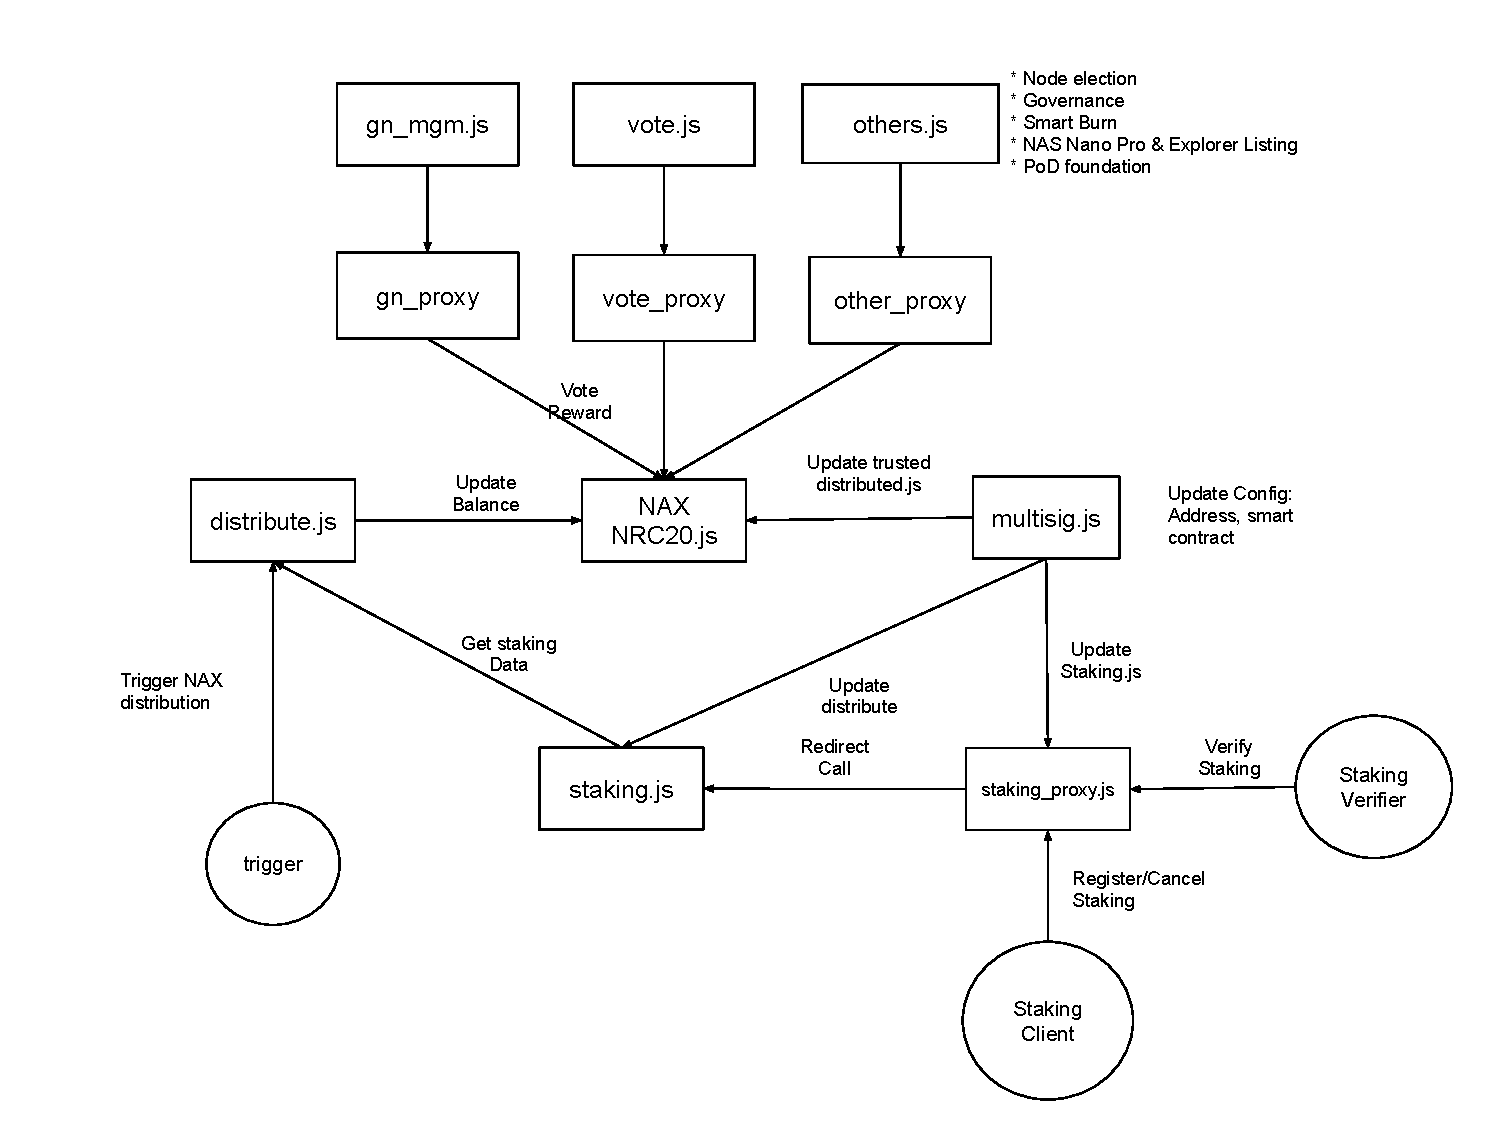
\includegraphics[width=0.8\textwidth]{../common/nax.pdf}
  \caption{NAX contract component schematic \label{fig:nax_framework}}
\end{figure}
